\documentclass[a4paper,twocolumn]{scrartcl}
\usepackage{fpr}

\addbibresource{biblography.bib} % Bibliographie einbinden

\setlist[itemize]{parsep=0pt}
\setlist[enumerate]{parsep=0pt}

\begin{document}
\selectlanguage{ngerman}
\twocolumn[{
  \title{Protokoll: M12}
  \firstAuthor{xxx}
  \secondAuthor{yyy}
  \setAbstract{%
	Der Abstract soll in kompakter Form den Inhalt einer wissenschaftlichen
	Arbeit wiedergeben. Er soll hier nicht mehr als 100 Worte umfassen. Diesen Teil
	Ihrer Arbeit kann jeder Interessent kostenlos lesen, bevor er den Artikel kauft.
	Umso wichtiger ist es, dem potentiellen Käufer kurz aber genau zu erklären, was
	er bekommt. Es gibt ein paar paper, die sich nur mit diesem Thema befassen, da
	aber ein Abstract keine Zitate enthält, werden diese im Text genannt.
  }
  \titleOfExperiment{Saitenschwingung}
  \dateOfExperiment{21.06.2021}
  \submissionDate{\today}
  \tutor{Joscha Hanel}
  \maketitle}]
  
\section*{Einleitung und Durchführung}
In dem Versuch wurde gezeigt, dass die Resonanzschwingungen stehende Wellen bilden und die Abhängigkeit der Frequenz von Mode $n$, Länge der Saite $l$ und Kraft $F_0$ ermittelt. Aus all dem konnte am Ende die lineare Massendichte $µ$ der Saite bestimmt werden.\\

Bei der Saitenschwingung wird eine Saite (S) zwischen 2 Punkten (Sp1,Sp2) eingespannt und zum Schwingen angeregt. Wichtig war hierbei die verstellbare Länge des schwingbaren Anteils der Saite durch zwei verschiebbare Reiter (R1, R2). Der zweite Aufhängepunkt (Sp2) war hierbei an einem Lasthebel (L) befestigt, der an fünf gleichmäßig verteilten Kerben eine Masse (M) halten konnte und um die Achse (A) drehbar war. Der erste Aufhängepunkt (Sp1) konnte durch eine Justierschraube (JS) fein in seiner Position eingestellt werden. Es wurden eine Erregerspule (ES) und eine Detektorspule (DS) unterhalb der Saite platziert um die Schwingung anzuregen und zu messen. Beide Spulen wurden dann zur simultanen Überprüfung an zwei Kanäle eines Oszilloskops angeschlossen. Zusätzlich wurde an der Erregerspule (ES) ein Tonfrequenz-Generator angeschlossen, um die Erregerfrequenz einstellen zu können.

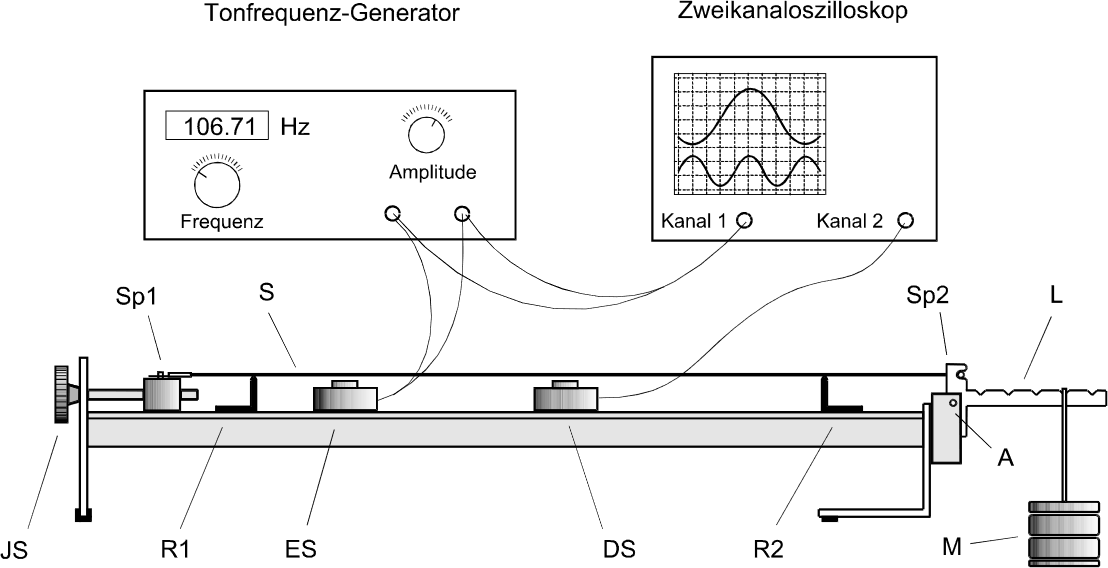
\includegraphics[width=3.25in]{Aufbau.png}
\caption{Abb.3 Versuchsanordnung aus dem Skript M12}

Da die Enden fest sind, können auf der Saiten nur stehende Wellen oder Linearkombination dieser existieren.
Bei einer stehenden Welle befinden sich Wellenberge und -täler immer an den gleichen Stellen und statt sich entlang der Saite auszubreiten, schwingt die stehende Welle nur nach oben und unten.\\
Damit eine reine stehende Welle entsteht, muss die Anregungsfrequenz der Eigenfrequenz der stehenden Welle entsprechen und die Anregung sollte an einem der Wellenberge passieren, da sonst zusätzlich höhere Frequenzen angeregt werden.\\
Die Frequenz $f$ einer Welle hängt im allgemeinen von der Wellenlänge $\lambda$ und der Phasengeschwindigkeit $c$ ab:\\
$$f = \frac{c}{\lambda}$$\\
Die Phasengeschwindigkeit ist dabei die Geschwindigkeit, mit der sich die Wellenberge einer Welle fester Frequenz bewegt.
Nicht zu verwechseln mit der Gruppengeschwindigkeit, die die Geschwindigkeit der Hülle einer beliebigen Welle angibt.\\
Bei einer festen Saitenlänge, lässt sich die Wellenlänge der stehenden Welle direkt aus der Länge der Saite $l$ und der Schwingungsmode $n$ berechnen:\\
$$\lambda = \frac{2l}{n}$$\\
$$f_n = \frac{nc}{2l}$$\\
Die Phasengeschwindigkeit für transversalen Wellen, die bei den stehende Wellen relevant ist, folgt aus Formel (6) der Versuchsbeschreibung $^{[1]}$:
$$f_n = \frac{n}{2l}\sqrt{\frac{F_0}{\mu}}$$\\
Hierbei ist $\mu$ die lineare Massendichte der Saite und $F_0$ die Spannkraft.\\

Da die Saite mit einem Elektromagneten angeregt wurde ist die effektive Anregungsfrequenz doppelt so groß, wie die am Funktionsgenerator eingestellte. Das liegt daran, dass die Saite schnell ihre Magnetisierung ändert und deswegen immer vom Elektromagneten angezogen wird, wenn dieser ein Maximum im Betrag durchläuft, während die Saite in den Nullstellen durch die Spannkraft zurückgezogen wird.\\

Nach jeder Messung wurde der Lasthebel neu eingestellt, sodass er parallel zum Boden ist. Da das ohne Anhaltspunkte in der Luft abgeschätzt wurde, ist das nicht sonderlich genau. Die Ungenauigkeit wurde auf 10° geschätzt.
Es finden 2 Kraftübertragungen statt:
1. Vom Gewicht auf den Hebel
2. Vom Hebel auf die Saite
In beiden Fällen geht jeweils ein Anteil von $1 - cos(\phi_{Soll} - \phi_{ist})$ verloren. Bei 10° ergibt sich daher ein Verlust von:\\
$$1-cos^2(10°) = 3\%$$














\section*{Ergebnisse}



















1.Welche  Näherungen  und  Idealisierungen  sind  in  der  obigen  Modellbetrachtung  zur Saitenschwingung enthalten? Welche davon sind experimentell nicht sicher zu realisieren bzw.  ggf.  „verletzt“?  Woran  könnte  man  Abweichungen  vom  Modell  in  der  Praxis  fest-stellen?
2.Erklären Sie die Entstehung des Signals an der Detektorspule! Wieso schwingt die Saite im  Resonanzfall  mit  der  doppelten  Erregerfrequenz? (Hinweis:  Der  Kern  beider  Spulen ist „weichmagnetisch“.)√
3.Ein  reales  Saiteninstrument  wie  z.B.  eine  Gitarre  wird  gewöhnlich  nicht  exakt  in  der Mitte der Saite „gespielt“ (angeregt): Welche Folgen hat das für den entstehenden Klang (Frequenzspektrum)?  Was  erwarten  Sie  bei  stärkerer und  „anharmonischer“  Anregung einer Saite? (√)
4.Was  versteht  man  unter  der  Phasengeschwindigkeit  einer  Welle?  Was  ist  „Gruppen-geschwindigkeit“?√
5.Welche  Bedingungen  müssen  für  die  Erzeugung  stehender  Wellen  erfüllt  werden?  Wie wird das (technisch) im Versuch realisiert? (√)
6.Warum  ist  die  Dämpfung  im  Versuch  sehr  schwach  und welche  Ursachen  hat  sie?  Wie würde sich eine stärkere Dämpfung auswirken?

	


\end{document}
